
\section{Results}\label{Sec:Results}

The results will be presented in two sections: First, the forecasting accuracy of the prediction models is evaluated and presented. Second, the results of the market simulation -- which is run once with the true consumption and production values and once with the predicted values -- are reported.


%%%%%%%%%%%%%%%%%%%%%%%%%%%%
%%%   Benchmark models   %%%
%%%%%%%%%%%%%%%%%%%%%%%%%%%%

\subsection{Evaluation of the prediction models}\label{Sec:Results;Subsec:Forecast}

Three prediction models where each applied to 82 consumer data sets and 12 prosumer data sets: the benchmark model (see Section~\ref{Sec:Method;Subsec:Benchmark}), the LSTM RNN model (see Section~\ref{Sec:Method;Subsec:LSTM}), and the LASSO model (see Section~\ref{Sec:Method;Subsec:LASSO}). All three prediction models are compared and evaluated using the error measures presented in Section~\ref{Sec:Method;Subsec:Error}.


%%%%%%%%%%%
\subsubsection{Consumption data}

The performance of the prediction values was tested on a quarter of the available data. That is, the prediction models were fitted on the consumption values from 01.01.2017 00:00 to 30.09.2017 00:00 which is equivalent to 131,040 data points per data set. For all 82 consumer data sets the models were fitted separately resulting in 82 distinct prediction models for each method. The fitted models were then used to make energy consumption predictions in 15-minute intervals on the data from 01.10.2017 00:00 to 01.01.2018 00:00. This equates to 8,836 predicted values per data set per model. The performance of the three prediction models according to five error measures is shown in Table~\ref{Tab:avg_errormeasures}.
%
\begingroup\catcode`"=9
\begin{table}[ht]
{\footnotesize
    \csvreader[centered tabular=l|SSSSS,
    before reading=\sisetup{round-mode=places,round-precision=4,round-integer-to-decimal},
    filter not strcmp={\thecsvinputline}{1},
    table head=
    \hline\hline
     \multicolumn{1} {l}{\textbf{Model}} & \multicolumn{1} {|c}{\textbf{MAE}} & \multicolumn{1} {c}{\textbf{RMSE}} & \multicolumn{1} {c}{\textbf{MAPE}} & \multicolumn{1} {c}{\textbf{NRSME}} & \multicolumn{1} {c}{\textbf{MASE}}\\
    \hline,
    no head,
    separator=comma,
    respect all,
    late after line=\\,
    table foot=\hline \hline]
    {thesis/tables/avg_errorMeasures.csv}{}%
    {\csvcolii & \csvcoliii & \csvcoliv & \csvcolv & \csvcolvi & \csvcolvii}}%
    \caption[Summary statistics of households' total consumption and production in 2017]{Summary statistics of households' total consumption and production in 2017. \quantnet\href{ }{BLEMdescStatEnergy}}
    \label{Tab:avg_errormeasures}
\end{table}
\endgroup

%%%%%%%%%%%
\subsubsection{Production data}




%%%%%%%%%%%%%%%%%%%%%%%%%%%%
%%%   Market simulation   %%%
%%%%%%%%%%%%%%%%%%%%%%%%%%%%

\subsection{Evaluation of the market simulation}\label{Sec:Results;Subsec:Simulation}



%%%%%%%%%%%
\subsubsection{True consumption and production values}



%%%%%%%%%%%
\subsubsection{Predicted consumption and production values}



%%%%%%%%%%%
\subsubsection{Cost due to prediction errors}



%%%%%%%%%%%%%%%%%%%%%%%%%%%%%%%%%%%%%%%%%%%%%%%%%%%%%%%%%%%%%%%%%

\begin{itemize}

    \item Organize material and present results.

    \item Use tables, figures (but prefer visual presentation):
        \begin{itemize}
            \item Tables and figures should supplement (and not duplicate) the
                text.

            \item Tables and figures should be provided with
            legends.\\
                {\it Figure~\ref{Fig:Resids} shows how to include and reference
                graphics. The graphic must be labelled before. Files must be in
                \texttt{.eps} format.}

                \begin{figure}[ht]
                \begin{center}
                    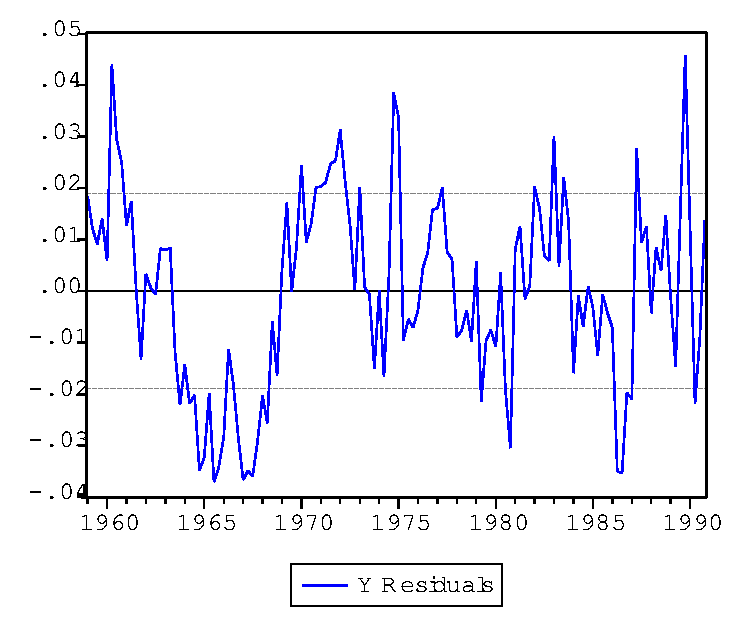
\includegraphics[scale=0.5,angle=0]{thesis/figures/graph.pdf}
                    \caption{Estimated residuals from model XXX. ...}
                    \label{Fig:Resids}
                \end{center}
                \end{figure}

            \item Tables and graphics may appear in the text or in
                the appendix, especially if there are many simulation results
                tabulated, but is also depends on the study and number of tables resp.
                figures. The key graphs and tables must appear in
                the text!
        \end{itemize}

    \item Latex is really good at rendering formulas:\\
        {\it Equation (\ref{Eq:SpecDens}) represents the ACs of a stationary
        stochastic process:
        \begin{equation}
            f_y(\lambda) = (2\pi)^{-1} \sum_{j=-\infty}^{\infty}
                           \gamma_j e^{-i\lambda j}
                         =(2\pi)^{-1}\left(\gamma_0 + 2 \sum_{j=1}^{\infty}
        \gamma_j \cos(\lambda j)\right)
                                        \label{Eq:SpecDens}
        \end{equation}
        where $i=\sqrt{-1}$ is the imaginary unit, $\lambda \in [-\pi,
        \pi]$ is the frequency and the $\gamma_j$ are the autocovariances
        of $y_t$.}

\newpage

    \item Discuss results:
        \begin{itemize}
            \item Do the results support or do they contradict economic theory ?
            \item What does the reader learn from the results?
            \item Try to give an intuition for your results.
            \item Provide robustness checks.
            \item Compare to previous research.
        \end{itemize}
\end{itemize}
